\documentclass[]{book}
\usepackage{lmodern}
\usepackage{amssymb,amsmath}
\usepackage{ifxetex,ifluatex}
\usepackage{fixltx2e} % provides \textsubscript
\ifnum 0\ifxetex 1\fi\ifluatex 1\fi=0 % if pdftex
  \usepackage[T1]{fontenc}
  \usepackage[utf8]{inputenc}
\else % if luatex or xelatex
  \ifxetex
    \usepackage{mathspec}
  \else
    \usepackage{fontspec}
  \fi
  \defaultfontfeatures{Ligatures=TeX,Scale=MatchLowercase}
\fi
% use upquote if available, for straight quotes in verbatim environments
\IfFileExists{upquote.sty}{\usepackage{upquote}}{}
% use microtype if available
\IfFileExists{microtype.sty}{%
\usepackage[]{microtype}
\UseMicrotypeSet[protrusion]{basicmath} % disable protrusion for tt fonts
}{}
\PassOptionsToPackage{hyphens}{url} % url is loaded by hyperref
\usepackage[unicode=true]{hyperref}
\hypersetup{
            pdftitle={Intro to R for High Schoolers},
            pdfauthor={Scott LaForest},
            pdfborder={0 0 0},
            breaklinks=true}
\urlstyle{same}  % don't use monospace font for urls
\usepackage{natbib}
\bibliographystyle{apalike}
\usepackage{color}
\usepackage{fancyvrb}
\newcommand{\VerbBar}{|}
\newcommand{\VERB}{\Verb[commandchars=\\\{\}]}
\DefineVerbatimEnvironment{Highlighting}{Verbatim}{commandchars=\\\{\}}
% Add ',fontsize=\small' for more characters per line
\usepackage{framed}
\definecolor{shadecolor}{RGB}{248,248,248}
\newenvironment{Shaded}{\begin{snugshade}}{\end{snugshade}}
\newcommand{\KeywordTok}[1]{\textcolor[rgb]{0.13,0.29,0.53}{\textbf{#1}}}
\newcommand{\DataTypeTok}[1]{\textcolor[rgb]{0.13,0.29,0.53}{#1}}
\newcommand{\DecValTok}[1]{\textcolor[rgb]{0.00,0.00,0.81}{#1}}
\newcommand{\BaseNTok}[1]{\textcolor[rgb]{0.00,0.00,0.81}{#1}}
\newcommand{\FloatTok}[1]{\textcolor[rgb]{0.00,0.00,0.81}{#1}}
\newcommand{\ConstantTok}[1]{\textcolor[rgb]{0.00,0.00,0.00}{#1}}
\newcommand{\CharTok}[1]{\textcolor[rgb]{0.31,0.60,0.02}{#1}}
\newcommand{\SpecialCharTok}[1]{\textcolor[rgb]{0.00,0.00,0.00}{#1}}
\newcommand{\StringTok}[1]{\textcolor[rgb]{0.31,0.60,0.02}{#1}}
\newcommand{\VerbatimStringTok}[1]{\textcolor[rgb]{0.31,0.60,0.02}{#1}}
\newcommand{\SpecialStringTok}[1]{\textcolor[rgb]{0.31,0.60,0.02}{#1}}
\newcommand{\ImportTok}[1]{#1}
\newcommand{\CommentTok}[1]{\textcolor[rgb]{0.56,0.35,0.01}{\textit{#1}}}
\newcommand{\DocumentationTok}[1]{\textcolor[rgb]{0.56,0.35,0.01}{\textbf{\textit{#1}}}}
\newcommand{\AnnotationTok}[1]{\textcolor[rgb]{0.56,0.35,0.01}{\textbf{\textit{#1}}}}
\newcommand{\CommentVarTok}[1]{\textcolor[rgb]{0.56,0.35,0.01}{\textbf{\textit{#1}}}}
\newcommand{\OtherTok}[1]{\textcolor[rgb]{0.56,0.35,0.01}{#1}}
\newcommand{\FunctionTok}[1]{\textcolor[rgb]{0.00,0.00,0.00}{#1}}
\newcommand{\VariableTok}[1]{\textcolor[rgb]{0.00,0.00,0.00}{#1}}
\newcommand{\ControlFlowTok}[1]{\textcolor[rgb]{0.13,0.29,0.53}{\textbf{#1}}}
\newcommand{\OperatorTok}[1]{\textcolor[rgb]{0.81,0.36,0.00}{\textbf{#1}}}
\newcommand{\BuiltInTok}[1]{#1}
\newcommand{\ExtensionTok}[1]{#1}
\newcommand{\PreprocessorTok}[1]{\textcolor[rgb]{0.56,0.35,0.01}{\textit{#1}}}
\newcommand{\AttributeTok}[1]{\textcolor[rgb]{0.77,0.63,0.00}{#1}}
\newcommand{\RegionMarkerTok}[1]{#1}
\newcommand{\InformationTok}[1]{\textcolor[rgb]{0.56,0.35,0.01}{\textbf{\textit{#1}}}}
\newcommand{\WarningTok}[1]{\textcolor[rgb]{0.56,0.35,0.01}{\textbf{\textit{#1}}}}
\newcommand{\AlertTok}[1]{\textcolor[rgb]{0.94,0.16,0.16}{#1}}
\newcommand{\ErrorTok}[1]{\textcolor[rgb]{0.64,0.00,0.00}{\textbf{#1}}}
\newcommand{\NormalTok}[1]{#1}
\usepackage{longtable,booktabs}
% Fix footnotes in tables (requires footnote package)
\IfFileExists{footnote.sty}{\usepackage{footnote}\makesavenoteenv{long table}}{}
\usepackage{graphicx,grffile}
\makeatletter
\def\maxwidth{\ifdim\Gin@nat@width>\linewidth\linewidth\else\Gin@nat@width\fi}
\def\maxheight{\ifdim\Gin@nat@height>\textheight\textheight\else\Gin@nat@height\fi}
\makeatother
% Scale images if necessary, so that they will not overflow the page
% margins by default, and it is still possible to overwrite the defaults
% using explicit options in \includegraphics[width, height, ...]{}
\setkeys{Gin}{width=\maxwidth,height=\maxheight,keepaspectratio}
\IfFileExists{parskip.sty}{%
\usepackage{parskip}
}{% else
\setlength{\parindent}{0pt}
\setlength{\parskip}{6pt plus 2pt minus 1pt}
}
\setlength{\emergencystretch}{3em}  % prevent overfull lines
\providecommand{\tightlist}{%
  \setlength{\itemsep}{0pt}\setlength{\parskip}{0pt}}
\setcounter{secnumdepth}{5}
% Redefines (sub)paragraphs to behave more like sections
\ifx\paragraph\undefined\else
\let\oldparagraph\paragraph
\renewcommand{\paragraph}[1]{\oldparagraph{#1}\mbox{}}
\fi
\ifx\subparagraph\undefined\else
\let\oldsubparagraph\subparagraph
\renewcommand{\subparagraph}[1]{\oldsubparagraph{#1}\mbox{}}
\fi

% set default figure placement to htbp
\makeatletter
\def\fps@figure{htbp}
\makeatother

\usepackage{booktabs}

\title{Intro to R for High Schoolers}
\author{Scott LaForest}
\date{2020-02-23}

\begin{document}
\maketitle

{
\setcounter{tocdepth}{1}
\tableofcontents
}
\chapter{Prerequisites}\label{prerequisites}

We will have to install a few things before we get started using R to
help us understand math and statistics.

\section{Install R}\label{install-r}

Download and install the most recent version of R.
\href{https://cran.rstudio.com/}{Install R}. If you are running the most
updated version of OSX you should be fine to select the first download
file, version 3.6.2.

\section{Install RStudio}\label{install-rstudio}

RStudion is the most popular integrated development environment (IDE)
for R.
\href{https://rstudio.com/products/rstudio/download/\#download}{Download
RStudio}. Again, if you are running the most updated version of OSX you
should be fine to download the most recent version of RStudio.

That's it, now you are ready to follow along with the walkthrough.

\chapter{Walkthrough}\label{walkthrough}

\section{What R you talking about?}\label{what-r-you-talking-about}

R is a programming language that is popular among mathematicians,
scientists, staticians, and many other professional careers that need to
analyze and understand large amounts of data. R and Python are the two
most popluar languages for working with data. If you plan on going into
a STEM field or plan to do any research you will most likely need to
have an understanding of how to program in one of these two languages.
Now is a great time to learn how to analyze data programmitically.

\section{Walkthrough}\label{walkthrough}

\subsection{R Basics}\label{r-basics}

We will start by playing around on the R Console. The console is in the
lower left portion of the screen and should have a line that is blank
except for a \texttt{\textgreater{}} symbol. Place your cursor next to
the \texttt{\textgreater{}} to start typing inputs for R to evaluate. R
can be used as a basic calculator. Try typing some mathematical
expressions then press enter and R will evaluate them.

Follow along by typing the following commands into the R console.

\begin{Shaded}
\begin{Highlighting}[]
\DecValTok{3} \OperatorTok{+}\StringTok{ }\DecValTok{4}
\end{Highlighting}
\end{Shaded}

\begin{verbatim}
## [1] 7
\end{verbatim}

\begin{Shaded}
\begin{Highlighting}[]
\DecValTok{1}\OperatorTok{/}\DecValTok{3}
\end{Highlighting}
\end{Shaded}

\begin{verbatim}
## [1] 0.3333333
\end{verbatim}

\begin{Shaded}
\begin{Highlighting}[]
\FloatTok{2.5} \OperatorTok{*}\StringTok{ }\DecValTok{3}
\end{Highlighting}
\end{Shaded}

\begin{verbatim}
## [1] 7.5
\end{verbatim}

Nothing too impressive yet but that's not all R can do. Think of a
mathematical function and try evaluating an expression.

\begin{Shaded}
\begin{Highlighting}[]
\KeywordTok{sqrt}\NormalTok{(}\DecValTok{64}\NormalTok{)}
\end{Highlighting}
\end{Shaded}

\begin{verbatim}
## [1] 8
\end{verbatim}

\begin{Shaded}
\begin{Highlighting}[]
\KeywordTok{cos}\NormalTok{(}\DecValTok{60}\NormalTok{)}
\end{Highlighting}
\end{Shaded}

\begin{verbatim}
## [1] -0.952413
\end{verbatim}

Oops, we just calculated the cos of 60 radians! Let's convert radians to
degrees.

\begin{Shaded}
\begin{Highlighting}[]
\KeywordTok{cos}\NormalTok{(}\DecValTok{60}\OperatorTok{*}\NormalTok{pi}\OperatorTok{/}\DecValTok{180}\NormalTok{)}
\end{Highlighting}
\end{Shaded}

\begin{verbatim}
## [1] 0.5
\end{verbatim}

So far we've seen how R can function as a calculator but R can do so
much more. Before we start working we need one more concept that will
help us in our calculations. The programming concept of variables. A
variable in programming acts as a bucket to hold a piece of data for
later use. The benefit of using a variable is that we can set it equal
to a value and use that value as many times as we want.

\begin{Shaded}
\begin{Highlighting}[]
\CommentTok{# This line is a comment and will not be interpreted by R}
\CommentTok{# We use comments to help explain what our code is doing, whatever comes after the # is ignored.}
\CommentTok{# The syntax for a variable is as follows var_name <- some_value}
\NormalTok{a <-}\StringTok{ }\DecValTok{5}
\CommentTok{# Notice when you run this chunk nothing prints out.}
\end{Highlighting}
\end{Shaded}

Now we can use \texttt{a} as many times as we want.

\begin{Shaded}
\begin{Highlighting}[]
\NormalTok{a}
\end{Highlighting}
\end{Shaded}

\begin{verbatim}
## [1] 5
\end{verbatim}

\begin{Shaded}
\begin{Highlighting}[]
\NormalTok{a}\OperatorTok{*}\DecValTok{3}
\end{Highlighting}
\end{Shaded}

\begin{verbatim}
## [1] 15
\end{verbatim}

\begin{Shaded}
\begin{Highlighting}[]
\NormalTok{b <-}\StringTok{ }\NormalTok{a}\OperatorTok{+}\DecValTok{3}
\end{Highlighting}
\end{Shaded}

\begin{Shaded}
\begin{Highlighting}[]
\NormalTok{b}
\end{Highlighting}
\end{Shaded}

\begin{verbatim}
## [1] 8
\end{verbatim}

That should be enough R for now. Lets move on to linear regression.

\subsection{Linear Regression with
MTcars}\label{linear-regression-with-mtcars}

Follow along via the R console. Our goal with the walkthrough is to look
at correlation between variables and use linear regression to predict or
infer meaning in the data. Let's start by looking at all the datasets
that come installed in R. The code below should open another tab with a
list of available datasets.

\begin{Shaded}
\begin{Highlighting}[]
\KeywordTok{data}\NormalTok{()}
\end{Highlighting}
\end{Shaded}

We will start by looking at some relationships between variables in the
mtcars dataset. Try the following code to learn more about the dataset.

\begin{Shaded}
\begin{Highlighting}[]
\NormalTok{?mtcars}
\end{Highlighting}
\end{Shaded}

Notice that we get the definition of each of the variables included in
the data set as well as the number of rows and variables. However, we do
not get any examples of the data. Now let's take a look at a subset of
the data.

\begin{Shaded}
\begin{Highlighting}[]
\KeywordTok{head}\NormalTok{(mtcars)}
\end{Highlighting}
\end{Shaded}

\begin{verbatim}
##                    mpg cyl disp  hp drat    wt  qsec vs am gear carb
## Mazda RX4         21.0   6  160 110 3.90 2.620 16.46  0  1    4    4
## Mazda RX4 Wag     21.0   6  160 110 3.90 2.875 17.02  0  1    4    4
## Datsun 710        22.8   4  108  93 3.85 2.320 18.61  1  1    4    1
## Hornet 4 Drive    21.4   6  258 110 3.08 3.215 19.44  1  0    3    1
## Hornet Sportabout 18.7   8  360 175 3.15 3.440 17.02  0  0    3    2
## Valiant           18.1   6  225 105 2.76 3.460 20.22  1  0    3    1
\end{verbatim}

Now we will try to select a variable to predict the mpg of a car. Before
we get into the analysis, we need to have a quick review of linear
regression. One of the most common types of linear regression is the
Least Squares Regression (LSR). The goal with LSR is to find the line
that minimizes the residuals between the points in the data and the LSR
line. Remember that the residuals are the difference between our
predicted value vs the actual. In the plot below the residuals are shown
as the red line from the actual data point to the predicted value on the
line. 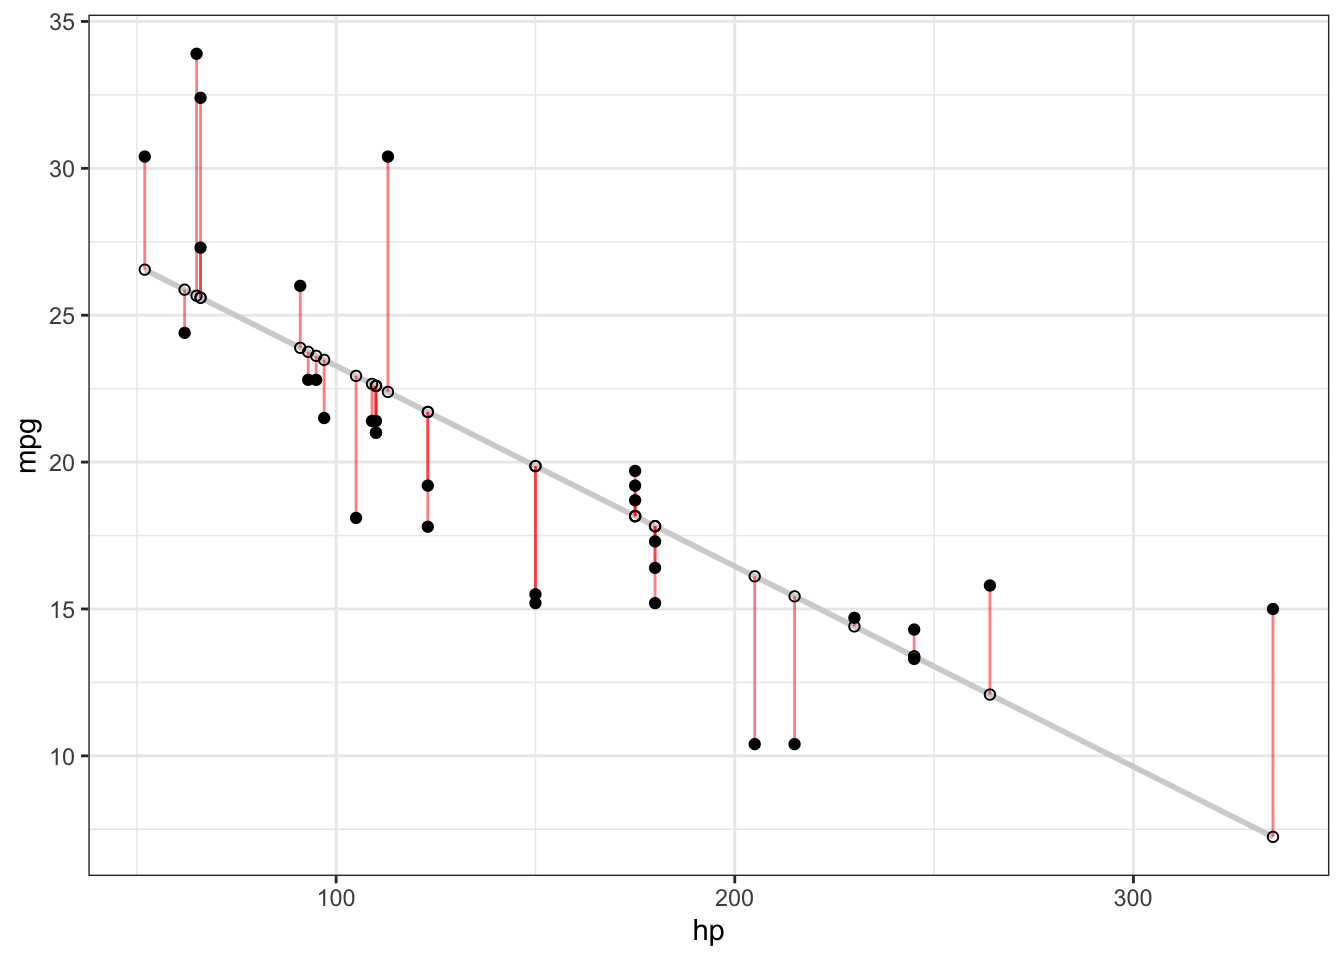
\includegraphics{ASDemo_files/figure-latex/unnamed-chunk-16-1.pdf}
The output of Least Squares Regression is a formula. In single variable
regression the formula should look very similar to a typical
slope-intercept form of an equation. \[y = \alpha + \beta \cdot x\]
where \(\alpha\) is the y-intercept of our LSR line and \(\beta\) is the
coefficient of our independent variable also known as the slope.
Remember that intuitively, \(\beta\) is the average increase or decrease
for our dependent (y) variable when our independent (x) variable changes
by one unit. R will do all of the work for us but it is useful to
remember how to calculate both \(\alpha\) and \(\beta\).

\[\beta = r \cdot \frac{S_y}{S_x}\] where \(r\) is the correlation
coefficient between \(y\) and \(x\), \(S_y\) is the standard deviation
of the \(y\) variable and \(S_x\) is the standard deviation of the \(x\)
variable.

\[\alpha = \overline y - \beta \cdot \overline x\] Now we have the
necessary equations to allow us to find the LSR line for a set of data.
If we had to, we could now compute the equation of the line of best fit
using the two formulas above. Before we find the regression formula we
need to find a variable that correlates well with our independent
variable, mpg. Our first task is to get an overview of how each variable
correlates with the mpg variable. A pairplot will give us a visual
overview of the correlation between the variables.

\begin{Shaded}
\begin{Highlighting}[]
\KeywordTok{pairs}\NormalTok{(mtcars)}
\end{Highlighting}
\end{Shaded}

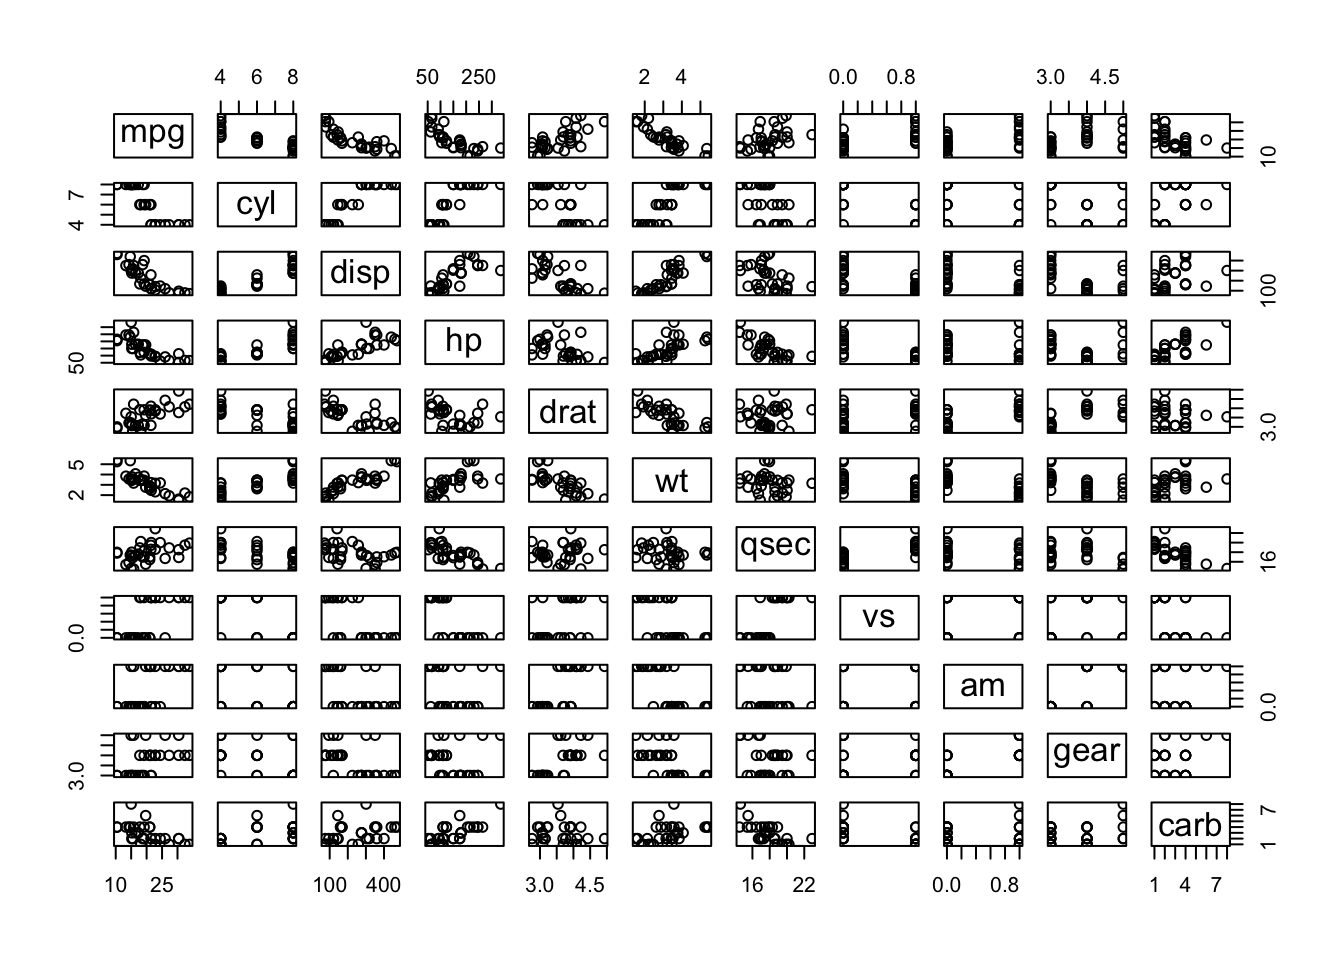
\includegraphics{ASDemo_files/figure-latex/unnamed-chunk-17-1.pdf} Whoa,
that's a lot of information. However, we are interested in predicting
mpg from a different dependent variable and we only need to look at the
first row. It seems that \texttt{wt}, \texttt{disp}, \texttt{cyl},
\texttt{drat},and \texttt{hp} might have some correlation with Temp.
Lets plot each relationship separately with the following code.

\begin{Shaded}
\begin{Highlighting}[]
\KeywordTok{plot}\NormalTok{(mtcars}\OperatorTok{$}\NormalTok{wt, mtcars}\OperatorTok{$}\NormalTok{mpg)}
\end{Highlighting}
\end{Shaded}

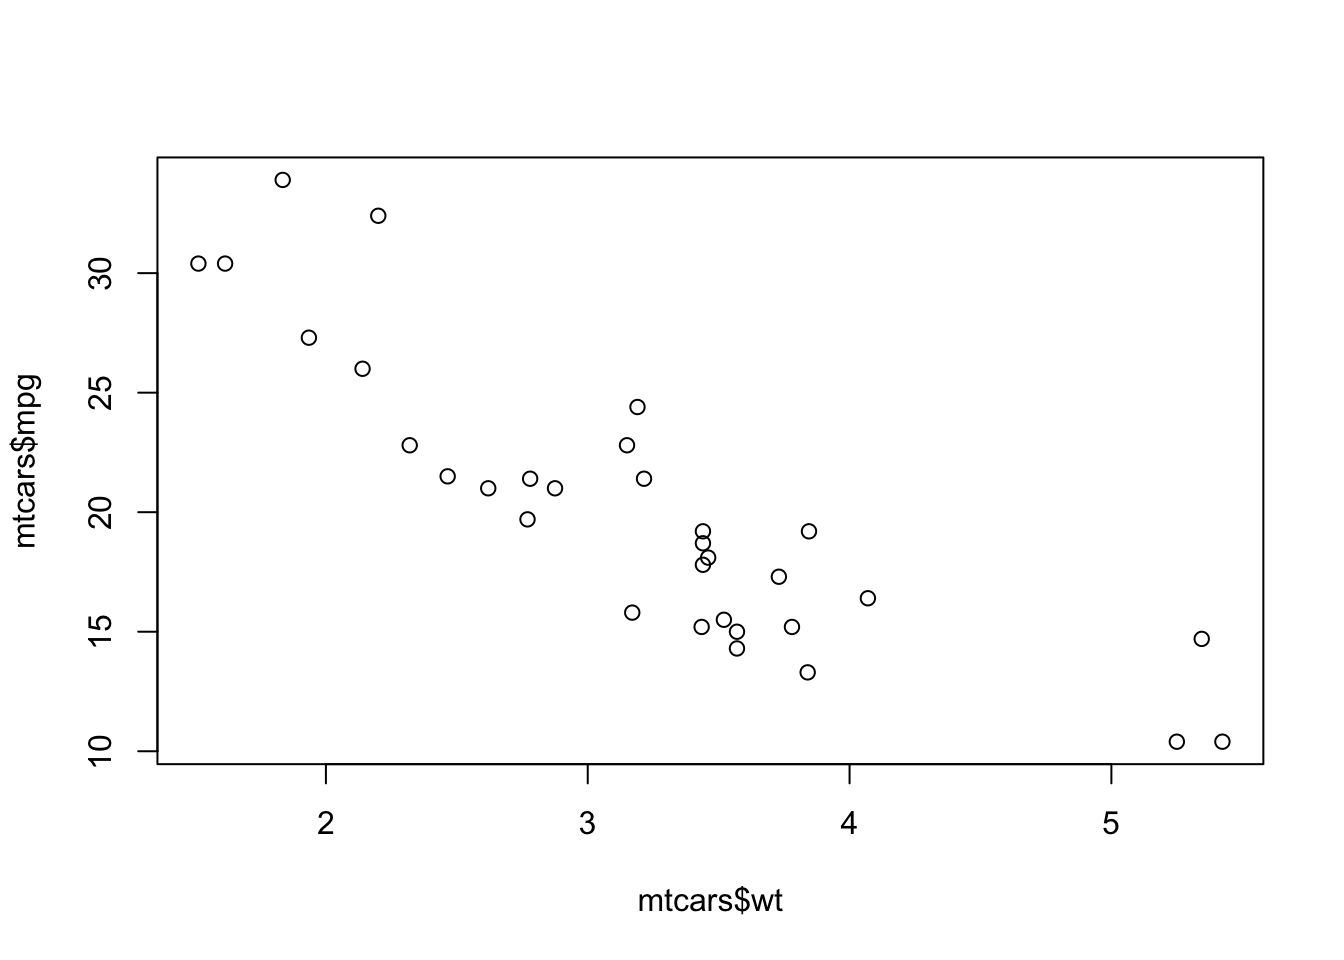
\includegraphics{ASDemo_files/figure-latex/unnamed-chunk-18-1.pdf}

\begin{Shaded}
\begin{Highlighting}[]
\KeywordTok{plot}\NormalTok{(mtcars}\OperatorTok{$}\NormalTok{disp, mtcars}\OperatorTok{$}\NormalTok{mpg)}
\end{Highlighting}
\end{Shaded}

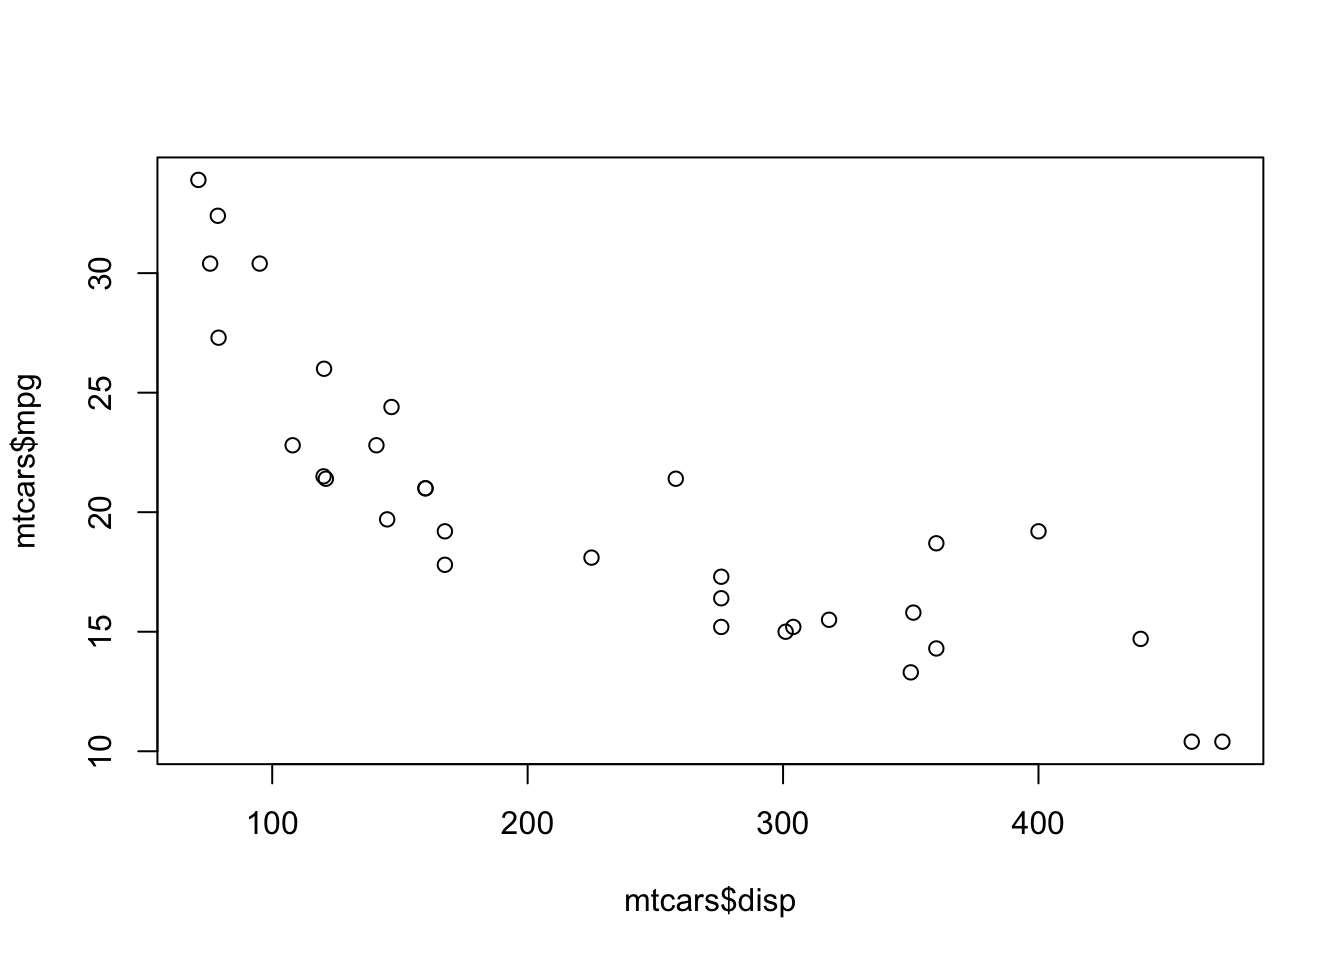
\includegraphics{ASDemo_files/figure-latex/unnamed-chunk-18-2.pdf}

\begin{Shaded}
\begin{Highlighting}[]
\KeywordTok{plot}\NormalTok{(mtcars}\OperatorTok{$}\NormalTok{hp, mtcars}\OperatorTok{$}\NormalTok{mpg)}
\end{Highlighting}
\end{Shaded}

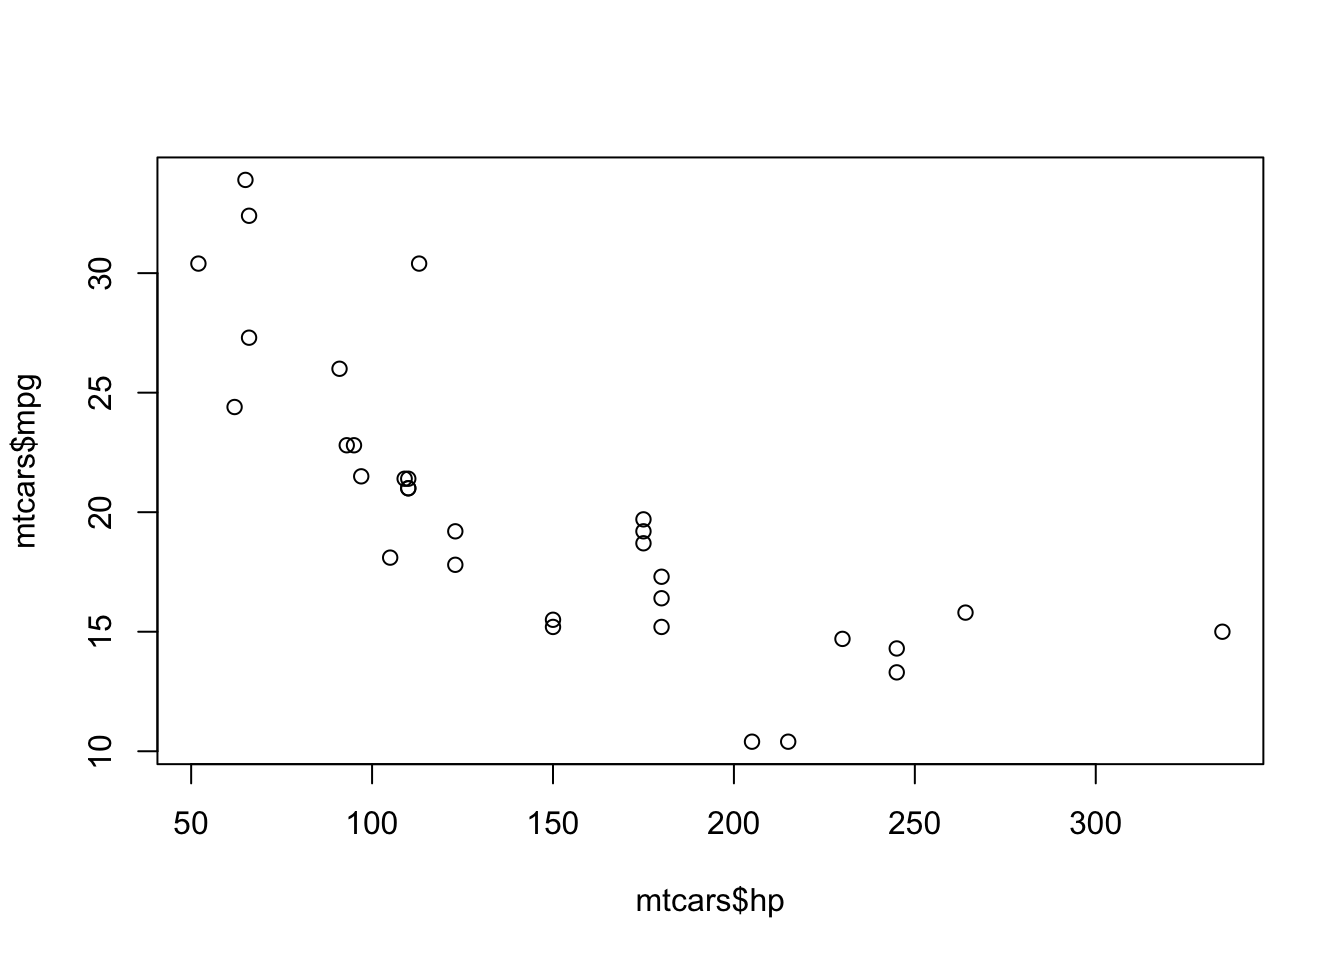
\includegraphics{ASDemo_files/figure-latex/unnamed-chunk-18-3.pdf}

\begin{Shaded}
\begin{Highlighting}[]
\KeywordTok{plot}\NormalTok{(mtcars}\OperatorTok{$}\NormalTok{cyl, mtcars}\OperatorTok{$}\NormalTok{mpg)}
\end{Highlighting}
\end{Shaded}

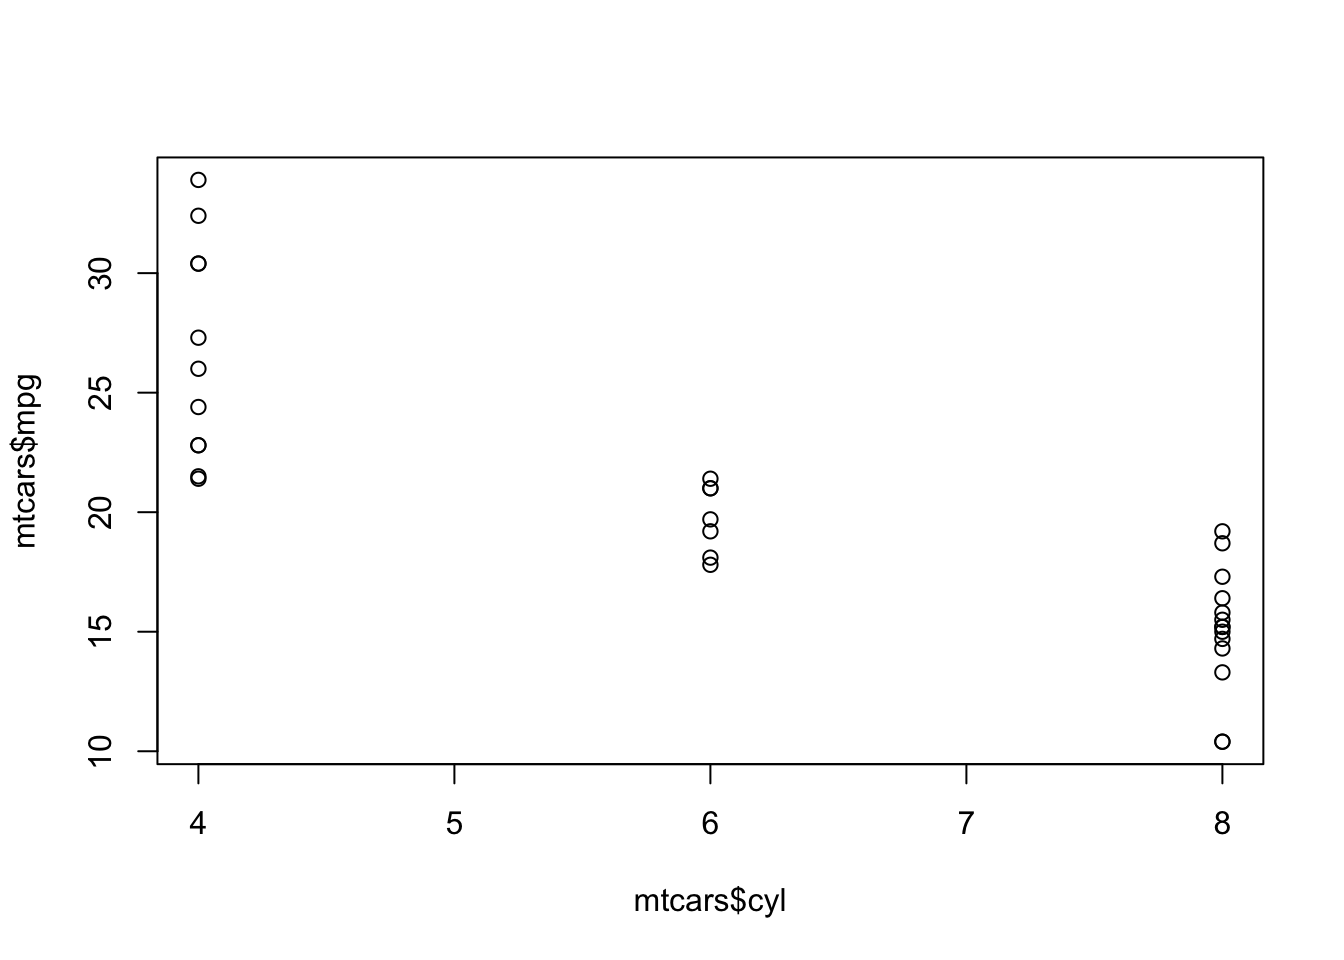
\includegraphics{ASDemo_files/figure-latex/unnamed-chunk-18-4.pdf}

\begin{Shaded}
\begin{Highlighting}[]
\KeywordTok{plot}\NormalTok{(mtcars}\OperatorTok{$}\NormalTok{drat, mtcars}\OperatorTok{$}\NormalTok{mpg)}
\end{Highlighting}
\end{Shaded}

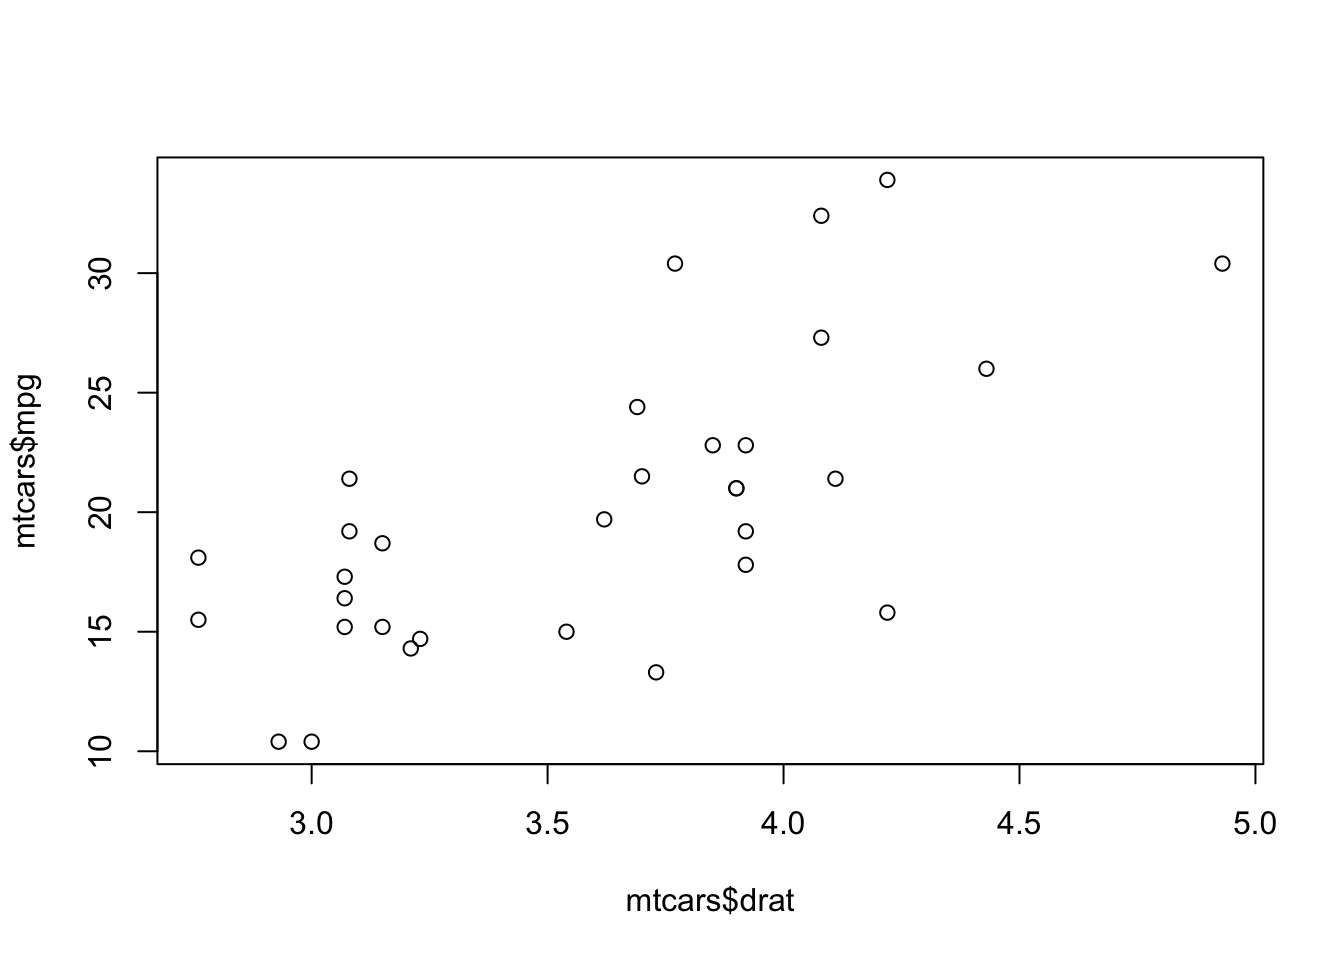
\includegraphics{ASDemo_files/figure-latex/unnamed-chunk-18-5.pdf} Which
plot seems to show the highest correlation? Possibly \texttt{wt} is the
highest negative correlation while \texttt{drat} seems to have a
slightly positive correlation. Lets use the correlation coefficient to
see for sure. The \texttt{cor()} function will calculate the correlation
coefficient for us. One side note, we need to include the
\texttt{use\ =\ \textquotesingle{}complete.obs\textquotesingle{}} option
to omit rows with blank values.

\begin{Shaded}
\begin{Highlighting}[]
\CommentTok{# cor without blanks and to make it easier to read only include the first row with [1,]}
\KeywordTok{cor}\NormalTok{(mtcars, }\DataTypeTok{use =} \StringTok{'complete.obs'}\NormalTok{)[}\DecValTok{1}\NormalTok{,]}
\end{Highlighting}
\end{Shaded}

\begin{verbatim}
##        mpg        cyl       disp         hp       drat         wt       qsec         vs         am       gear       carb 
##  1.0000000 -0.8521620 -0.8475514 -0.7761684  0.6811719 -0.8676594  0.4186840  0.6640389  0.5998324  0.4802848 -0.5509251
\end{verbatim}

Lets use some variables to help us calculate \(\alpha\) and \(\beta\).

\begin{Shaded}
\begin{Highlighting}[]
\CommentTok{# r can be calculated using the cor() function}
\NormalTok{r <-}\StringTok{ }\KeywordTok{cor}\NormalTok{(}\DataTypeTok{x =}\NormalTok{ mtcars}\OperatorTok{$}\NormalTok{wt, }\DataTypeTok{y =}\NormalTok{ mtcars}\OperatorTok{$}\NormalTok{mpg)}
\CommentTok{# sd() calculates the standard deviation}
\NormalTok{sx <-}\StringTok{ }\KeywordTok{sd}\NormalTok{(mtcars}\OperatorTok{$}\NormalTok{wt)}
\NormalTok{sy <-}\StringTok{ }\KeywordTok{sd}\NormalTok{(mtcars}\OperatorTok{$}\NormalTok{mpg)}
\NormalTok{beta <-}\StringTok{ }\NormalTok{r}\OperatorTok{*}\NormalTok{(sy}\OperatorTok{/}\NormalTok{sx)}
\NormalTok{beta}
\end{Highlighting}
\end{Shaded}

\begin{verbatim}
## [1] -5.344472
\end{verbatim}

\begin{Shaded}
\begin{Highlighting}[]
\NormalTok{ybar <-}\StringTok{ }\KeywordTok{mean}\NormalTok{(mtcars}\OperatorTok{$}\NormalTok{mpg)}
\NormalTok{xbar <-}\StringTok{ }\KeywordTok{mean}\NormalTok{(mtcars}\OperatorTok{$}\NormalTok{wt)}
\NormalTok{alpha <-}\StringTok{ }\NormalTok{ybar }\OperatorTok{-}\StringTok{ }\NormalTok{beta}\OperatorTok{*}\NormalTok{xbar}
\NormalTok{alpha}
\end{Highlighting}
\end{Shaded}

\begin{verbatim}
## [1] 37.28513
\end{verbatim}

Now because I'm evil I decided to wait until the end to show a shortcut
to calculate the equation of the LSR line. The lm() function allows us
to do all of the above steps, and more, in one step. Look at the help
documentation for the \texttt{lm()} function.

\begin{Shaded}
\begin{Highlighting}[]
\NormalTok{?lm}
\end{Highlighting}
\end{Shaded}

To use the \texttt{lm()} function, it is best to save the outcome in a
variable. Also, the function parameter is a little weird and the syntax
for the function parameter is
\texttt{(dependent\_variable\ \textasciitilde{}\ independent\_variable)}.

\begin{Shaded}
\begin{Highlighting}[]
\NormalTok{model <-}\StringTok{ }\KeywordTok{lm}\NormalTok{(mtcars}\OperatorTok{$}\NormalTok{mpg }\OperatorTok{~}\StringTok{ }\NormalTok{mtcars}\OperatorTok{$}\NormalTok{wt)}
\end{Highlighting}
\end{Shaded}

To see the outcome of our linear model we can use the \texttt{summary()}
function.

\begin{Shaded}
\begin{Highlighting}[]
\KeywordTok{summary}\NormalTok{(model)}
\end{Highlighting}
\end{Shaded}

\begin{verbatim}
## 
## Call:
## lm(formula = mtcars$mpg ~ mtcars$wt)
## 
## Residuals:
##     Min      1Q  Median      3Q     Max 
## -4.5432 -2.3647 -0.1252  1.4096  6.8727 
## 
## Coefficients:
##             Estimate Std. Error t value Pr(>|t|)    
## (Intercept)  37.2851     1.8776  19.858  < 2e-16 ***
## mtcars$wt    -5.3445     0.5591  -9.559 1.29e-10 ***
## ---
## Signif. codes:  0 '***' 0.001 '**' 0.01 '*' 0.05 '.' 0.1 ' ' 1
## 
## Residual standard error: 3.046 on 30 degrees of freedom
## Multiple R-squared:  0.7528, Adjusted R-squared:  0.7446 
## F-statistic: 91.38 on 1 and 30 DF,  p-value: 1.294e-10
\end{verbatim}

We can plot the line on top of our scatter plot to see our handywork!

\begin{Shaded}
\begin{Highlighting}[]
\KeywordTok{plot}\NormalTok{(mtcars}\OperatorTok{$}\NormalTok{wt, mtcars}\OperatorTok{$}\NormalTok{mpg)}
\KeywordTok{abline}\NormalTok{(model)}
\end{Highlighting}
\end{Shaded}

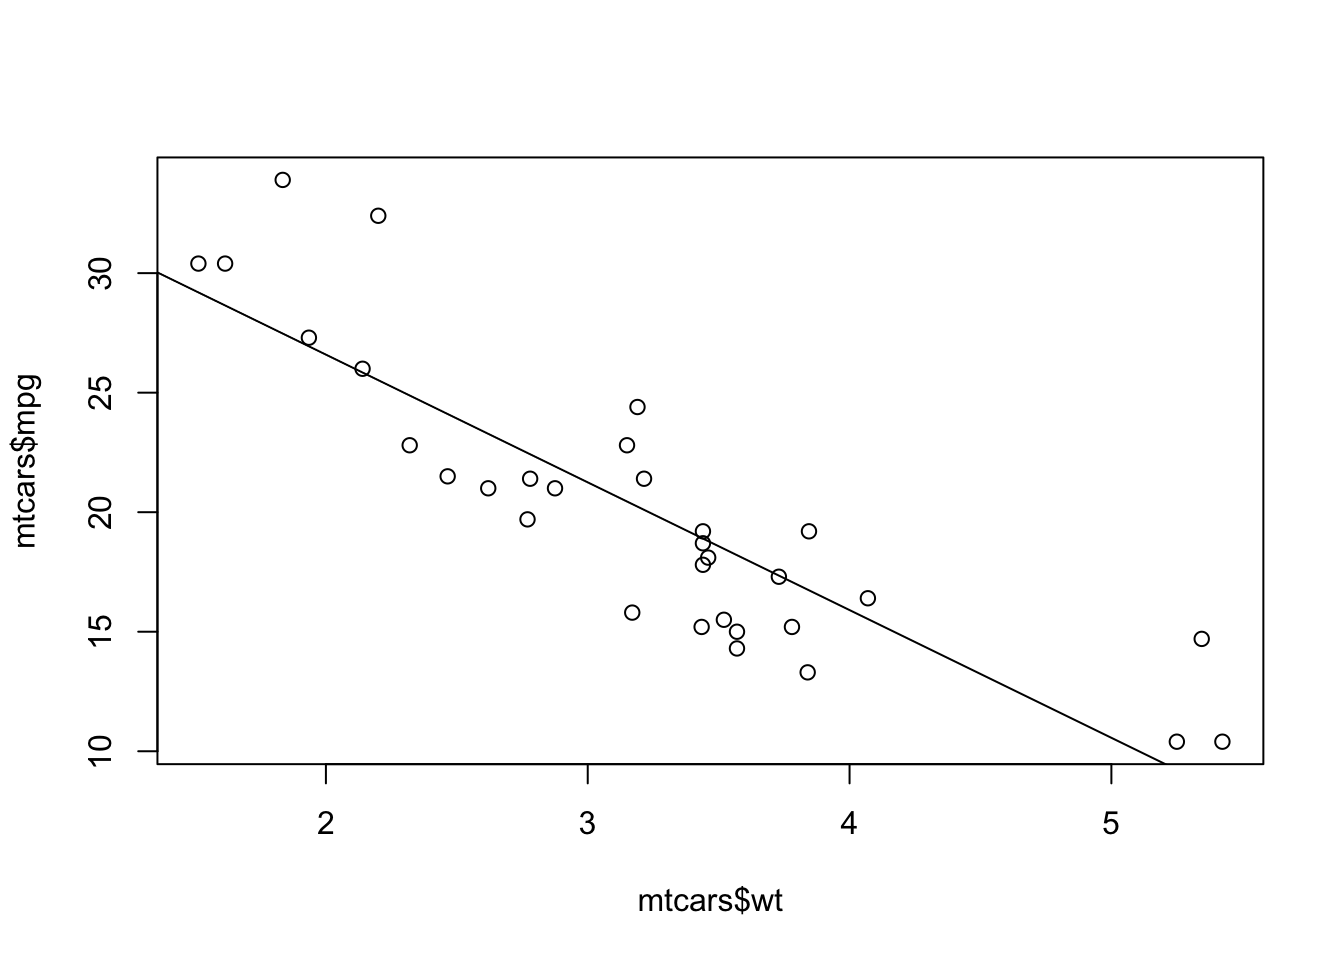
\includegraphics{ASDemo_files/figure-latex/unnamed-chunk-25-1.pdf}

\chapter{Minilab}\label{minilab}

\section{R Markdown Intro}\label{r-markdown-intro}

This is an R Markdown document. Markdown is a simple formatting syntax
for authoring HTML, PDF, and MS Word documents. For more details on
using R Markdown see \url{http://rmarkdown.rstudio.com}.

The way we will use it is to prove your R skills and apply what we have
learned so far. The great thing about R Markdown is that you can type
regular text as well as run R commands. R markdown files have
\texttt{chunks} that let you run R in the same document. Try it below by
checking the available datasets by calling the \texttt{data()} function.
Type in \texttt{data()} and press the run (little green triangle) button
on the chunk.

\begin{Shaded}
\begin{Highlighting}[]
\KeywordTok{data}\NormalTok{()}
\end{Highlighting}
\end{Shaded}

To complete this minilab you will need to type your code and answers in
the code chunks. You have already run some code but you can answer
questions by typing your answer between the single quotes and run the
chunk.

\subsection{\texorpdfstring{Q1: What is the description for the
\texttt{airquality}
dataset?}{Q1: What is the description for the airquality dataset?}}\label{q1-what-is-the-description-for-the-airquality-dataset}

\begin{Shaded}
\begin{Highlighting}[]
\NormalTok{description <-}\StringTok{ 'New York Air Quality Measurements'}
\KeywordTok{print}\NormalTok{(description)}
\end{Highlighting}
\end{Shaded}

\begin{verbatim}
## [1] "New York Air Quality Measurements"
\end{verbatim}

The rest of the minilab will require you to type either an answer or
some code in every code chunk.

Let's continue by exploring the \texttt{airquality} dataset. Type in the
code to call for help on the dataset.

\begin{Shaded}
\begin{Highlighting}[]
\CommentTok{# type your code on the line below}
\end{Highlighting}
\end{Shaded}

\subsection{\texorpdfstring{Q2: How many observations and how many
variables are included in the \texttt{airquality}
dataset?}{Q2: How many observations and how many variables are included in the airquality dataset?}}\label{q2-how-many-observations-and-how-many-variables-are-included-in-the-airquality-dataset}

\begin{Shaded}
\begin{Highlighting}[]
\CommentTok{# Type your answers between the '' for each answer.}
\NormalTok{observations <-}\StringTok{ ''}
\NormalTok{variables <-}\StringTok{ ''}
\CommentTok{# Do not type below this line}
\KeywordTok{paste}\NormalTok{(}\StringTok{'There are '}\NormalTok{ , observations , }\StringTok{' observations and '}\NormalTok{ , variables, }\StringTok{' variables.'}\NormalTok{)}
\end{Highlighting}
\end{Shaded}

\begin{verbatim}
## [1] "There are    observations and    variables."
\end{verbatim}

Take a look at the first five rows of the \texttt{airquality} dataset.

Lets look at the correlation between each of the variables. Remember to
only include complete observations.

\section{Q3: What variable has the highest correlation with the Temp
variable? What is the correlation
coefficient?}\label{q3-what-variable-has-the-highest-correlation-with-the-temp-variable-what-is-the-correlation-coefficient}

\begin{Shaded}
\begin{Highlighting}[]
\NormalTok{variable_name <-}\StringTok{ ''}
\NormalTok{cor_coeff <-}\StringTok{ ''}

\CommentTok{# Do not type below this line}
\KeywordTok{paste}\NormalTok{( variable_name , }\StringTok{'is the most highly correlated with Temp and has a correlation coefficient of'}\NormalTok{ , cor_coeff)}
\end{Highlighting}
\end{Shaded}

\begin{verbatim}
## [1] " is the most highly correlated with Temp and has a correlation coefficient of "
\end{verbatim}

Lets look at the correlation in a more visual manner. Plot the a
scatterplot of each variable in the dataset, also known as a pair plot.

\subsection{Q4: Which row and column seems to show the best correlation
with Temp with Temp as the independent
variable?}\label{q4-which-row-and-column-seems-to-show-the-best-correlation-with-temp-with-temp-as-the-independent-variable}

\begin{Shaded}
\begin{Highlighting}[]
\NormalTok{row_num <-}\StringTok{ ''}
\NormalTok{col_num <-}\StringTok{ ''}

\CommentTok{# Do not type below this line}
\KeywordTok{paste}\NormalTok{(}\StringTok{'Row X Column:'}\NormalTok{,row_num,}\StringTok{"X"}\NormalTok{,col_num, }\StringTok{'which is'}\NormalTok{, }\KeywordTok{colnames}\NormalTok{(airquality)[}\KeywordTok{as.numeric}\NormalTok{(row_num)], }\StringTok{'and'}\NormalTok{, }\KeywordTok{colnames}\NormalTok{(airquality)[}\KeywordTok{as.numeric}\NormalTok{(col_num)] )}
\end{Highlighting}
\end{Shaded}

\begin{verbatim}
## [1] "Row X Column:  X  which is NA and NA"
\end{verbatim}

Pair plots are can be hard to read. Plot a scatter plot for Ozone vs
Temp, Solar.R vs Temp, and Wind vs Temp.

Finally, we need to fit a regression line to our data. Choosing the
independent variable that is most correlated, fit a model and print out
the summary of the model.

\subsection{\texorpdfstring{Q5: What are the \(\alpha\) and \(\beta\)
values for your
regression?}{Q5: What are the \textbackslash{}alpha and \textbackslash{}beta values for your regression?}}\label{q5-what-are-the-alpha-and-beta-values-for-your-regression}

\begin{Shaded}
\begin{Highlighting}[]
\NormalTok{alpha <-}\StringTok{ ''}
\NormalTok{beta <-}\StringTok{ ''}

\KeywordTok{paste}\NormalTok{(}\StringTok{'Your equation is y = '}\NormalTok{, alpha, }\StringTok{' + '}\NormalTok{ , beta, }\StringTok{'X'}\NormalTok{, }\DataTypeTok{sep =} \StringTok{""}\NormalTok{)}
\end{Highlighting}
\end{Shaded}

\begin{verbatim}
## [1] "Your equation is y =  + X"
\end{verbatim}

\subsection{Q6: What is the R\^{}2 value? What does this tell
us?}\label{q6-what-is-the-r2-value-what-does-this-tell-us}

\begin{Shaded}
\begin{Highlighting}[]
\NormalTok{r2 <-}\StringTok{ ''}
\NormalTok{meaning <-}\StringTok{ ''}

\KeywordTok{paste}\NormalTok{(}\StringTok{'R^2 ='}\NormalTok{ , r2,}\StringTok{'and'}\NormalTok{, meaning)}
\end{Highlighting}
\end{Shaded}

\begin{verbatim}
## [1] "R^2 =  and "
\end{verbatim}

\chapter{Swirl Minilab}\label{swirllab}

\section{R Packages}\label{r-packages}

We need to install a package before so that we can complete a minilab.
We can think of a package like an app on our phone. When you first turn
on a new phone you have the basic functionality that all other phones
have. If you need more functionality, you install new apps. Packages are
to R as apps are to your phone's operating system. The
\href{https://swirlstats.com/students.html}{swirl} package is a great
way to learn how to use the R programming language. Install the package,
run it, and learn R in the R console! Before we start we need to
download a swirl course that we can use to test our understanding so
far.
\href{https://github.com/scottyla19/as-r-intro/blob/master/AS_Intro_to_R.swc?raw=true}{Download
this file} so we can use it later.

Type the following code in the console. Notice once you start typing
RStudio provides hints. You can press \texttt{tab} to select the
function you want. We need to first download and install the package
with \texttt{install.packages()} function.

\begin{Shaded}
\begin{Highlighting}[]
\KeywordTok{install.packages}\NormalTok{(}\StringTok{'swirl'}\NormalTok{)}
\end{Highlighting}
\end{Shaded}

The code above will start a process that will download and install the
necessary parts so that we can use the swirl package.

Once the package is installed we need to tell R to use it with the
\texttt{library()} function.

\begin{Shaded}
\begin{Highlighting}[]
\KeywordTok{library}\NormalTok{(swirl)}
\end{Highlighting}
\end{Shaded}

Next, we need to install the course that we downloaded from above. The
\texttt{install\_course()} function will allow us to select a file to
install as a course. Type the following command into the console and
then find the \texttt{AS\_Intro\_to\_R.swc} file. The file should be in
your Downloads folder.

\begin{Shaded}
\begin{Highlighting}[]
\KeywordTok{install_course}\NormalTok{()}
\end{Highlighting}
\end{Shaded}

Now we can start the swirl app with the \texttt{swirl()} function. The
swirl program will ask you questions, allow you to type your answer, and
provide feedback, all in the R console.

\begin{Shaded}
\begin{Highlighting}[]
\KeywordTok{swirl}\NormalTok{()}
\end{Highlighting}
\end{Shaded}

Answer the initial setup questions and be sure to choose the ``AS Intro
to R'' course. The course covers the topics we discussed in the
walkthrough. Good Luck!

\bibliography{book.bib,packages.bib}

\end{document}
